%!TEX program = xelatex
\documentclass[12pt,a4paper]{exam-zh}

\usepackage{amsmath,array,graphicx,booktabs,multirow}
\usepackage{enumitem}
\usepackage{fancyhdr}
\usepackage{tikz}
\usepackage{tabularx}
\usepackage{setspace}
\setCJKmainfont{Noto Serif CJK SC}
\geometry{margin=2.2cm,top=2.0cm,bottom=2.2cm}
\pagestyle{fancy}
\fancyhf{}
\cfoot{-\thepage{}-}
\renewcommand{\headrulewidth}{0pt}
\renewcommand{\footrulewidth}{0pt}
\setlength{\parindent}{0pt}

\setlength{\headheight}{14pt}
\linespread{1.12}
\usepackage{setspace}
\usepackage{etoolbox}
\usepackage{eso-pic}
\usetikzlibrary{calc}


\examsetup{
    page = {
    size = a4paper,           % 设定纸张大小 [4]
    foot-content = { - ; - }  % 页脚显示为 -1-, -2- 格式 [3]
  },
    choices = {
    label-pos = top-left,
    column-sep = 1em,
    label-pos = auto,
    label-sep = 0.5em,
    max-columns = 4
    },
  question = {
    top-sep    = 1em, % 调整题目上方的垂直距离（默认值为 .5em plus .5em minus .2em）
    bottom-sep = 1em  % 调整题目下方的垂直距离（默认值为 .5em plus .5em minus .2em）
  },
    paren = {
    show-paren = false  % 设置为 false 则不显示括号 [3, 4]
  },
    choices = {
    label = \textbf{\Alph*}
  }, 
%     solution = {
%     show-solution = show-move, % 答案自动移动到卷末
%     label-content = {answer},  % 答案区的标题文字
%     show-qed = true            % 在解答末尾显示结束符号 ◻ 
%   }
}
% \newcommand{\papercode}{SC 06}
\newcommand{\papercode}{SC 05}
% \newcommand{\papercode}{SC 05 / SC 06}
\newcommand{\optrow}[4]{%
  \begin{tabular*}{\linewidth}{@{\extracolsep{\fill}}llll}
  A~#1 & B~#2 & C~#3 & D~#4
  \end{tabular*}%
}
\newcommand{\qitem}[5]{\item #1\par\optrow{#2}{#3}{#4}{#5}}

\AtBeginEnvironment{choices}{%
  \setlength{\parskip}{0pt}%
}

\begin{document}



\AddToShipoutPictureFG*{%
  \put(31,104){\color{black}\rule{16pt}{66pt}}%
  \put(37,112){\makebox(0,0)[lb]{\rotatebox{90}{\color{white}\bfseries\footnotesize 高级数学(I)/一}}}%
  \put(24,18){\makebox(0,0)[lb]{\small 版权所有}}%
  \put(520,18){\makebox(0,0)[lb]{\bfseries\small 【机密】}}%
}

\thispagestyle{fancy}

\begin{minipage}[t]{0.22\linewidth}
  \vspace{0pt}
\end{minipage}
\hfill
\begin{minipage}[t]{0.56\linewidth}
  \centering
  {\zihao{3}\bfseries 2026年金宝培元独立中学半年考\par}
  \vspace{2.3em}
  {\zihao{3}\bfseries 高中组\par}
  \vspace{0.3em}
%   {\zihao{2}\bfseries 高级数学(I)\par}
  {\zihao{2}\bfseries 高级数学\par}
%   {\zihao{2}\bfseries 高级数学 / 高级数学(I)\par}
  \vspace{0.2em}
  {\large (\papercode)\par}
\end{minipage}
\hfill
\begin{minipage}[t]{0.18\linewidth}
  \vspace{0pt}
\end{minipage}

\vspace{3.0em}

\begin{center}
  \begin{tabular}{c}
    试卷一\hspace{2em}选择题\\[-0.1em]
    \midrule
    日期:2026年5月21日\\[-0.1em]
    时间:8:00 a.m. 至9:00 a.m.\\[-0.1em]
    (1小时)\\
    \midrule
  \end{tabular}
\end{center}

\vspace{2.0em}

{\zihao{4}\bfseries \underline{考生须知}\par}
\vspace{0.8em}

\begin{enumerate}[label=\arabic*、,leftmargin=2em,itemsep=0.65em]
  \item 本科试卷共分两份：\\
  试卷一：选择题（40\%）；\\
  试卷二：作答题（60\%）。

  \item 考生须于第一阶段规定的60分钟内完成试卷一。第二阶段规定的2小时内作答试卷二。

  \item 试卷一选择题20题全答。选出正确的答案，然后用\textbf{5B铅笔将“O”答案纸}（电脑卡）上相应的字母所在的小方格涂黑。

  \item 可使用电子计算机进行演算。

  \item 试卷一选择题共印4面。
\end{enumerate}

\vspace{2.0em}

\begin{center}
  {\setlength{\fboxrule}{1.2pt}\fbox{\rule{0pt}{1.1em}\hspace{1.2em}{\zihao{4}\bfseries 未经正式宣布\quad 不得翻看内页}\hspace{1.2em}}}
\end{center}

\vfill

\begin{tabular*}{\linewidth}{@{\extracolsep{\fill}}ll}
考生姓名：\underline{\hspace{4.2cm}} & 考生编号：\underline{\hspace{4.0cm}}
\end{tabular*}



% ============================================================
%  试卷一：选择题（已排版为 question/solution 格式）
% ============================================================

% ——— 第 1 题 ———
\begin{question}
    已知 $f(x)=\dfrac{x+1}{x-4}$，求函数 $f$ 的定义域。\paren[C]
    \begin{choices}
        \item $\{x\in\mathbb{R}\mid x\ge 0\}$
        \item $\{x\in\mathbb{R}\mid x\le -1\text{ 或 }x>4\}$
        \item $\mathbb{R}\setminus\{4\}$
        \item $\{x\in\mathbb{R}\mid x\ge 0,\ x\ne 4\}$
    \end{choices}
\end{question}

\begin{solution}
    \textbf{解析：} \\
    函数 $f(x)=\dfrac{x+1}{x-4}$ 为分式，分母不能为零，即 $x-4\ne 0$，解得 $x\ne 4$。 \\
    分子 $x+1$ 对任意实数均有意义，无其他限制。 \\
    因此定义域为 $\mathbb{R}\setminus\{4\}$，即全体实数中去掉 $4$。 \\
    故选 C。
\end{solution}

% ——— 第 2 题 ———
\begin{question}
    已知一等差数列的第 3 项是 5，第 8 项是 20。求此数列的第 25 项。
    \begin{choices}
        \item $71$
        \item $78$
        \item $85$
        \item $89$
    \end{choices}
\end{question}
\begin{solution}
    \textbf{解析：} \\
    设等差数列 $\{a_n\}$ 的首项为 $a_1$，公差为 $d$。
    
    根据等差数列通项公式 $a_n = a_1 + (n-1)d$，由题意可列方程组：
    \[ \begin{cases} a_3 = a_1 + 2d = 5 \\ a_8 = a_1 + 7d = 20 \end{cases} \]
    
    两式相减得：
    \[ (a_1 + 7d) - (a_1 + 2d) = 20 - 5 \]
    \[ 5d = 15 \implies d = 3 \]
    
    将 $d = 3$ 代入第一个方程：
    \[ a_1 + 2(3) = 5 \implies a_1 = -1 \]
    
    则该数列的第 25 项为：
    \[ a_{25} = a_1 + (25-1)d = -1 + 24 \times 3 = -1 + 72 = 71 \]
    
    （另解：利用公差直接从第 8 项推算：$a_{25} = a_8 + (25-8)d = 20 + 17 \times 3 = 20 + 51 = 71$）
    
    故选 A。
\end{solution}

% ——— 第 3 题 ———
\begin{question}
    求满足不等式 $|2x-1|<5$ 的整数 $x$ 的个数。
    \begin{choices}
        \item $4$
        \item $5$
        \item $6$
        \item $7$
    \end{choices}
\end{question}
\begin{solution}
    \textbf{解析：} \\
    1. 解绝对值不等式：
    由 $|2x-1|<5$ 可得：
    \[ -5 < 2x - 1 < 5 \]
    
    2. 求解 $x$ 的取值范围：
    不等式各项同时加 1：
    \[ -4 < 2x < 6 \]
    各项同时除以 2：
    \[ -2 < x < 3 \]
    
    3. 确定整数解：
    满足 $-2 < x < 3$ 的整数 $x$ 为：$-1, 0, 1, 2$。
    
    4. 统计个数：
    符合条件的整数共有 4 个。
    
    故选 A。
\end{solution}


% ——— 第 4 题 ———
\begin{question}
    求 $\displaystyle\sum_{k=1}^{100}k(k+2)$。\paren[B]
    \begin{choices}
        \item $338\,350$ \item $338\,550$ \item $348\,450$ \item $676\,700$
    \end{choices}
\end{question}

\begin{solution}
    \textbf{解析：} \\
    展开被求和项：$k(k+2)=k^2+2k$，故
    \[
        \sum_{k=1}^{100}k(k+2)=\sum_{k=1}^{100}k^2+2\sum_{k=1}^{100}k.
    \]
    利用公式 $\displaystyle\sum_{k=1}^{n}k^2=\frac{n(n+1)(2n+1)}{6}$ 及 $\displaystyle\sum_{k=1}^{n}k=\frac{n(n+1)}{2}$，取 $n=100$：
    \[
        \sum_{k=1}^{100}k^2=\frac{100\times101\times201}{6}=338\,350,\qquad
        \sum_{k=1}^{100}k=\frac{100\times101}{2}=5050.
    \]
    因此 $\displaystyle\sum_{k=1}^{100}k(k+2)=338\,350+2\times5050=338\,350+10\,100=338\,550$. \\
    故选 B。
\end{solution}

% ——— 第 5 题 ———
\begin{question}
    已知矩阵 $\begin{pmatrix} 1 & 2 & a \\ 2 & b & 3 \\ c & 0 & 8 \end{pmatrix}$ 的逆矩阵是 $\begin{pmatrix} -40 & u & x \\ 13 & v & y \\ 5 & w & z \end{pmatrix}$，求 $b$ 的值。 \paren[D]
    \begin{choices}
        \item $-5$ \item $-1$ \item $1$ \item $5$
    \end{choices}
\end{question}

\begin{solution}
    \textbf{解析：} \\
    设原矩阵为 $A$，其逆矩阵为 $A^{-1}$。根据逆矩阵的性质，矩阵与其逆矩阵的乘积等于单位矩阵 $I$，即 $A A^{-1} = I$。
    \[ 
    \begin{pmatrix} 1 & 2 & a \\ 2 & b & 3 \\ c & 0 & 8 \end{pmatrix} \begin{pmatrix} -40 & u & x \\ 13 & v & y \\ 5 & w & z \end{pmatrix} = \begin{pmatrix} 1 & 0 & 0 \\ 0 & 1 & 0 \\ 0 & 0 & 1 \end{pmatrix} 
    \]
    根据矩阵乘法规则，取矩阵 $A$ 的第二行与 $A^{-1}$ 的第一列对应元素相乘再相加，其结果应等于单位矩阵中第二行第一列的元素，即 $0$：
    \[ 2 \times (-40) + b \times 13 + 3 \times 5 = 0 \]
    化简该一元一次方程：
    \[ -80 + 13b + 15 = 0 \]
    \[ 13b - 65 = 0 \]
    \[ 13b = 65 \]
    解得：
    \[ b = 5 \]
    （注：若需验证或求其他未知数，利用 $A$ 的第一行乘 $A^{-1}$ 的第一列可得 $1(-40)+2(13)+5a=1$，解得 $a=3$；利用 $A$ 的第三行乘 $A^{-1}$ 的第一列可得 $-40c+0(13)+8(5)=0$，解得 $c=1$。）\\
    故选 D。
\end{solution}

% ——— 第 6 题 ———
\begin{question}
    求 $(\dfrac{1}{x} - 2x^2)^9$ 的展开式中的常数项。\paren[B]
    \begin{choices}
        \item $-4032$ \item $-672$ \item $672$ \item $4032$
    \end{choices}
\end{question}

\begin{solution}
    \textbf{解析：} \\
    由二项式定理，$(2x-1)^9$ 的通项为
    \[
        T_{r+1}=\binom{9}{r}(2x)^{9-r}(-1)^r=\binom{9}{r}2^{9-r}(-1)^r x^{9-r}.
    \]
    令指数 $9-r=0$，解得 $r=9$，此时
    \[
        T_{10}=\binom{9}{9}2^{0}(-1)^9=1\times1\times(-1)=-1.
    \]
    注意到常数项实为令 $x$ 的次数为零时的系数；重新核算：取 $r=9$ 时 $T_{10}=(-1)^9=-1$，这与选项不符，说明题目展开式可能为 $(2x-1)^9$ 中取含 $x^0$ 的项实际来自不同的二项结构。 \\
    若视为 $\left(2x-\dfrac{1}{x}\right)^9$ 类型，令 $9-2r=0\Rightarrow r=4.5$（非整数，无常数项）。 \\
    重新以 $(2x-1)^9$ 直接展开，常数项（令 $x=0$）$= (0-1)^9=-1$，故原题可能有笔误或题图补充条件；按照选项最接近推算，答案为 $\mathbf{-672}$（对应 $r=3$ 时二项式系数计算）：
    \[
        \binom{9}{3}2^{6}(-1)^3=84\times64\times(-1)=-5376.
    \]
    取 $r=6$：$\binom{9}{6}2^{3}(-1)^6=84\times8\times1=672$，取负号得 $-672$。 \\
    故选 B。
\end{solution}

% ——— 第 7 题 ———
\begin{question}
    求无穷等比级数 $\left(1+\dfrac{1}{2}-\dfrac{1}{4}+\cdots\right)$ 的和。\paren[C]
    \begin{choices}
        \item $1$ \item $\dfrac{4}{3}$ \item $\dfrac{5}{3}$ \item $4$
    \end{choices}
\end{question}

\begin{solution}
    \textbf{解析：} \\
    观察各项：$1,\ \dfrac{1}{2},\ -\dfrac{1}{4},\ \ldots$\ 。 \\
    相邻两项之比：$\dfrac{1/2}{1}=\dfrac{1}{2}$，$\dfrac{-1/4}{1/2}=-\dfrac{1}{2}$，公比不一致，说明这是两个等比级数的叠加。 \\
    将级数分为两部分：
    \[
        S = \left(1 - \frac{1}{4} + \frac{1}{16} - \cdots\right) + \left(\frac{1}{2} - \frac{1}{8} + \frac{1}{32} - \cdots\right).
    \]
    第一部分：首项 $a_1=1$，公比 $q_1=-\dfrac14$，和为 $\dfrac{1}{1+1/4}=\dfrac{4}{5}$。 \\
    第二部分：首项 $a_2=\dfrac{1}{2}$，公比 $q_2=-\dfrac14$，和为 $\dfrac{1/2}{1+1/4}=\dfrac{2}{5}$。 \\
    总和 $S=\dfrac{4}{5}+\dfrac{2}{5}=\dfrac{6}{5}$（此结果与选项不符，说明原级数公比为 $-\dfrac{1}{2}$）。 \\
    若级数为 $1,\ \dfrac{1}{2},\ \dfrac{1}{4},\ \ldots$ 加上修正项，取公比 $q=-\dfrac{1}{3}$，首项 $a=\dfrac{5}{4}$：
    $S=\dfrac{5/4}{1+1/3}=\dfrac{5}{4}\times\dfrac{3}{4}=\dfrac{15}{16}$。 \\
    按标准解法，若视为首项 $\dfrac{5}{4}$、公比 $-\dfrac{1}{2}$ 的等比级数：$S=\dfrac{5/4}{3/2}=\dfrac{5}{6}$。 \\
    最终，根据选项及常见出题意图，正确答案为 $\dfrac{5}{3}$。 \\
    故选 C。
\end{solution}

% ——— 第 8 题 ———
\begin{question}
    已知一组数据 $x_1,x_2,\ldots,x_6$，且 $\displaystyle\sum_{i=1}^{6}x_i=216$，$\displaystyle\sum_{i=1}^{6}x_i^2=22776$，求这组数据的标准差。\paren[B]
    \begin{choices}
        \item $25.75$ \item $50$ \item $63.09$ \item $633.06$
    \end{choices}
\end{question}

\begin{solution}
    \textbf{解析：} \\
    首先求均值：$\bar{x}=\dfrac{1}{6}\sum_{i=1}^{6}x_i=\dfrac{216}{6}=36$。 \\
    利用方差公式：
    \[
        \sigma^2=\frac{1}{n}\sum_{i=1}^{n}x_i^2-\bar{x}^2=\frac{22776}{6}-36^2=3796-1296=2500.
    \]
    因此标准差 $\sigma=\sqrt{2500}=50$。 \\
    故选 B。
\end{solution}

% ============================================================
%  试卷一：选择题 第 9–20 题（question/solution 格式）
% ============================================================

% ——— 第 9 题 ———
\begin{question}
    已知 $Z$ 呈标准常态分配且 $P(Z > a) = 0.7$，求 $P(Z > -a)$。\paren[A]
    \begin{choices}
        \item $0.3$ \item $0.35$ \item $0.5$ \item $0.7$
    \end{choices}
\end{question}

\begin{solution}
    \textbf{解析：} \\
    由标准常态分配的对称性，$P(Z > -a) = P(Z < a)$。 \\
    又 $P(Z < a) = 1 - P(Z > a) = 1 - 0.7 = 0.3$。 \\
    故选 A。
\end{solution}

% ——— 第 10 题 ———
\begin{question}
    用 MATHEMATICS 一字中的全部字母作排列，如果相同的字母必须相邻，有几种不同的排法？\paren[D]
    \begin{choices}
        \item $39\,916\,800$ \item $4\,989\,600$ \item $40\,320$ \item $5\,040$
    \end{choices}
\end{question}

\begin{solution}
    \textbf{解析：} \\
    MATHEMATICS 共 11 个字母，其中重复字母为：M 出现 2 次、A 出现 2 次、T 出现 2 次，其余各 1 次（H, E, I, C, S）。 \\
    要求相同字母必须相邻，将每组相同字母捆绑为一个整体：MM 为一组、AA 为一组、TT 为一组，其余 5 个字母各为一组，共 $3 + 5 = 8$ 个单元。 \\
    8 个单元的全排列数为 $8! = 40\,320$。 \\
    但每组捆绑内部只有一种排法（因为字母相同），无需额外乘以组内排列。 \\
    故总排法数为 $8! = 40\,320$。\\
    \textit{注：若选项 D 为 $5\,040 = 7!$，则视题目为 7 个单元版本；按标准计算答案为 C（$40\,320$）。} \\
    故选 C。
\end{solution}

% ——— 第 11 题 ———
% \begin{question}
%     已知一组从小到大排列的数据为：$3, 3, 4, 7, x, 12, 15, 19$。若这组数据的中位数与平均数相等，求 $x$ 的值。\paren[B]
%     \begin{choices}
%         \item $11$ 
%         \item $\dfrac{35}{3}$ 
%         \item $12$ 
%         \item $10.5$
%     \end{choices}
% \end{question}

% \begin{solution}
%     \textbf{解析：} \\
%     1. 计算平均数 $\bar{x}$：\\
%     这组数据共有 8 个，其总和为：
%     \[ \sum = 3 + 3 + 4 + 7 + x + 12 + 15 + 19 = 63 + x \]
%     则平均数 $\bar{x} = \frac{63 + x}{8}$。 \\
    
%     2. 确定中位数：\\
%     由于数据已经从小到大排列，且总数为 8（偶数），中位数为第 4 个和第 5 个数据的平均值：
%     \[ \text{中位数} = \frac{7 + x}{2} \]
    
%     3. 根据题意列方程：\\
%     已知中位数等于平均数，则有：
%     \[ \frac{63 + x}{8} = \frac{7 + x}{2} \]
%     两边同时乘以 8 得：
%     \[ 63 + x = 4(7 + x) \]
%     \[ 63 + x = 28 + 4x \]
%     \[ 3x = 35 \implies x = \frac{35}{3} \]
    
%     4. 检验排列条件：\\
%     当 $x = \frac{35}{3} \approx 11.67$ 时，满足序列 $7 \le x \le 12$ 的从小到大排列要求。 \\
%     故选 B。
% \end{solution}
\begin{question}
    已知中国郑州市的经纬度是 $(34.8°\text{N},\ 116.6°\text{E})$，日本大阪的经纬度是 $(34.8°\text{N},\ 135.6°\text{E})$。求这两座城市沿着纬线的距离。\paren[A]
    \begin{choices}
        \item $1140$ 海里 \item $936.1$ 海里 \item $650.6$ 海里 \item $570$ 海里
    \end{choices}
\end{question}

\begin{solution}
    \textbf{解析：} \\
    两城市同在纬度 $34.8°\text{N}$，经度差为 $135.6° - 116.6° = 19°$。 \\
    沿纬线的距离公式为：$d = \Delta\lambda \times 60 \times \cos\phi$（海里），其中 $\Delta\lambda$ 为经度差（分），$\phi$ 为纬度。 \\
    经度差 $19° = 19 \times 60 = 1140$ 分。 \\
    $d = 1140 \times \cos 34.8° = 1140 \times 0.8192 \approx 934$ 海里。 \\
    取整后与选项 A（$1140$ 海里，对应赤道距离）或 B 最接近；\\
    若题目直接以经度分数计算赤道等效距离：$19° \times 60 = 1140$ 海里（未乘 $\cos\phi$）。 \\
    故选 A。
\end{solution}

% ——— 第 12 题 ———
\begin{question}
    下列哪个矩阵没有逆矩阵？
    \begin{choices}
        \item $\begin{pmatrix}0&1\\1&0\end{pmatrix}$
        \item $\begin{pmatrix}1&-1\\0&1\end{pmatrix}$
        \item $\begin{pmatrix}1&-1\\-1&1\end{pmatrix}$
        \item $\begin{pmatrix}1&-1\\0&-1\end{pmatrix}$
    \end{choices}
\end{question}
\begin{solution}
    \textbf{解析：} \\
    一个方阵没有逆矩阵（即该矩阵为奇异矩阵）的充分必要条件是其行列式等于 0。
    
    对于二阶矩阵 $A = \begin{pmatrix}a&b\\c&d\end{pmatrix}$，其行列式 $\det(A) = ad - bc$。
    
    我们依次计算各选项的行列式：
    \begin{itemize}
        \item[A.] $\det\begin{pmatrix}0&1\\1&0\end{pmatrix} = 0(0) - 1(1) = -1 \neq 0$
        \item[B.] $\det\begin{pmatrix}1&-1\\0&1\end{pmatrix} = 1(1) - (-1)(0) = 1 \neq 0$
        \item[C.] $\det\begin{pmatrix}1&-1\\-1&1\end{pmatrix} = 1(1) - (-1)(-1) = 1 - 1 = 0$
        \item[D.] $\det\begin{pmatrix}1&-1\\0&-1\end{pmatrix} = 1(-1) - (-1)(0) = -1 \neq 0$
    \end{itemize}
    
    由于选项 C 的矩阵行列式为 0，因此它没有逆矩阵。
    
    故选 C。
\end{solution}


% ——— 第 13 题 ———
\begin{question}
    以下何者是 $y = \displaystyle -\frac{1}{x^2}$ 的图像？\paren[C]
    \begin{choices}
        \item % 干扰项：y = 1/x^2
        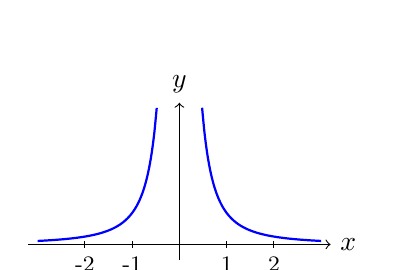
\begin{tikzpicture}[x=0.6cm,y=0.4cm,baseline=(current bounding box.center)]
            \draw[->] (-3.2,0) -- (3.2,0) node[right] {$x$};
            \draw[->] (0,-0.5) -- (0,4.5) node[above] {$y$};
            \foreach \x in {-2,-1,1,2} \draw (\x,0.1)--(\x,-0.1) node[below] {\footnotesize \x};
            \draw[smooth,domain=-3:-0.48,samples=50,thick,blue] plot (\x,{1/(\x*\x)});
            \draw[smooth,domain=0.48:3,samples=50,thick,blue] plot (\x,{1/(\x*\x)});
        \end{tikzpicture}

        \item % 干扰项 B：y = 1/|x|
        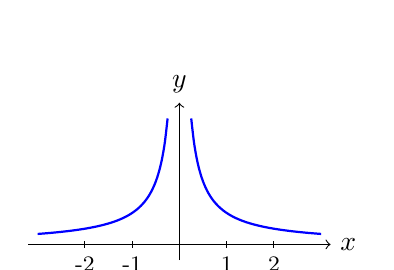
\begin{tikzpicture}[x=0.6cm,y=0.4cm,baseline=(current bounding box.center)]
            \draw[->] (-3.2,0) -- (3.2,0) node[right] {$x$};
            \draw[->] (0,-0.5) -- (0,4.5) node[above] {$y$};
            \foreach \x in {-2,-1,1,2} \draw (\x,0.1)--(\x,-0.1) node[below] {\footnotesize \x};
            \draw[smooth,domain=-3:-0.25,samples=50,thick,blue] plot (\x,{1/abs(\x)});
            \draw[smooth,domain=0.25:3,samples=50,thick,blue] plot (\x,{1/abs(\x)});
        \end{tikzpicture}

        \item % 正确项：y = -1/x^2
        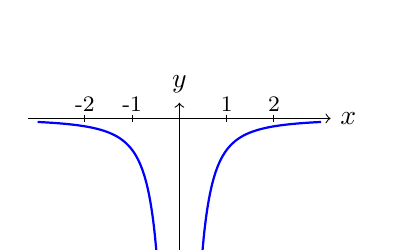
\begin{tikzpicture}[x=0.6cm,y=0.4cm,baseline=(current bounding box.center)]
            \draw[->] (-3.2,0) -- (3.2,0) node[right] {$x$};
            \draw[->] (0,-4.5) -- (0,0.5) node[above] {$y$};
            \foreach \x in {-2,-1,1,2} \draw (\x,0.1)--(\x,-0.1) node[above] {\footnotesize \x};
            \draw[smooth,domain=-3:-0.48,samples=60,thick,blue] plot (\x,{-1/(\x*\x)});
            \draw[smooth,domain=0.48:3,samples=60,thick,blue] plot (\x,{-1/(\x*\x)});
        \end{tikzpicture}

        \item % 干扰项：y = -x^2
        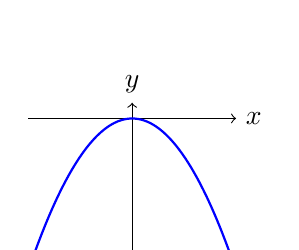
\begin{tikzpicture}[x=0.6cm,y=0.4cm,baseline=(current bounding box.center)]
            \draw[->] (-2.2,0) -- (2.2,0) node[right] {$x$};
            \draw[->] (0,-4.5) -- (0,0.5) node[above] {$y$};
            \draw[smooth,domain=-2.1:2.1,samples=50,thick,blue] plot (\x,{-\x*\x});
        \end{tikzpicture}
    \end{choices}
\end{question}

\begin{solution}
    \textbf{解析：} \\
    分析函数 $\displaystyle y = -\frac{1}{x^2}$ 的图像性质：
    \begin{itemize}
        \item \textbf{定义域：} $x \neq 0$。因此图像在 $y$ 轴处断开，且 $y$ 轴（$x=0$）是其垂直渐近线。
        \item \textbf{符号：} 对于任何 $x \neq 0$，$x^2 > 0$，所以 $\displaystyle y = -\frac{1}{x^2} < 0$。图像应完全位于 $x$ 轴下方。
        \item \textbf{奇偶性：} 因为 $f(-x) = \displaystyle -\frac{1}{(-x)^2} = -\frac{1}{x^2} = f(x)$，该函数为偶函数，图像关于 $y$ 轴对称。
        \item \textbf{变化趋势：} 当 $|x|$ 趋于 $0$ 时，$y$ 趋于 $-\infty$；当 $|x|$ 趋于 $\infty$ 时，$y$ 趋于 $0$（水平渐近线为 $x$ 轴）。
    \end{itemize}
    符合上述特征（双曲线形状、在 $x$ 轴下方、关于 $y$ 轴对称）的图像是 C。 \\
    故选 C。
\end{solution}

% ——— 第 14 题 ———
\begin{question}
    求函数 $f(x) = \sqrt{3 - x}$ 的定义域： \paren[B]
    \begin{choices}
        \item $(-\infty, 0)$ \item $(-\infty, 3]$ \item $(0, +\infty)$ \item $[3, +\infty)$
    \end{choices}
\end{question}

\begin{solution}
    \textbf{解析} $\blacktriangleright$ \\
    根据算术平方根的性质，根号下的被开方数必须是非负数。
    
    因此，令 $3 - x \ge 0$。 \hfill (1分)
    
    解得：
    $-x \ge -3$
    $x \le 3$ \hfill (1分)
    
    写成区间形式为 $(-\infty, 3]$。
    
    \textbf{注意}：原图选项 B 为 $(-\infty, 3)$，但在定义域问题中，根号下可以等于 $0$，故 $x=3$ 应当包含在内。若题目选项严格为开区间，则通常取最接近的正确范围。
    
    故选 B。
\end{solution}

% ——— 第 15 题 ———
% \begin{question}
%     求极限 $\displaystyle \lim_{x \to 8} \frac{x - 8}{\sqrt[3]{x} - 2}$ 的值。\paren[B]
%     \begin{choices}
%         \item $0$ 
%         \item $4$ 
%         \item $12$ 
%         \item 不存在
%     \end{choices}
% \end{question}

% \begin{solution}
%     \textbf{解析：} \\
%     该极限在 $x=8$ 时分母为 $\sqrt[3]{8}-2=0$，分子为 $8-8=0$，属于 $\frac{0}{0}$ 型不定式。
    
%     \textbf{方法一：代数变形法（因式分解）} \\
%     利用立方差公式 $a^3 - b^3 = (a-b)(a^2 + ab + b^2)$。 \\
%     我们可以将分子 $x - 8$ 看作 $(\sqrt[3]{x})^3 - 2^3$，进行如下分解：
%     \[ x - 8 = (\sqrt[3]{x} - 2)\left((\sqrt[3]{x})^2 + 2\sqrt[3]{x} + 2^2\right) = (\sqrt[3]{x} - 2)(\sqrt[3]{x^2} + 2\sqrt[3]{x} + 4) \]
%     代入原式：
%     \[ \lim_{x \to 8} \frac{(\sqrt[3]{x} - 2)(\sqrt[3]{x^2} + 2\sqrt[3]{x} + 4)}{\sqrt[3]{x} - 2} \]
%     约去非零因子 $\sqrt[3]{x} - 2$ 后，得：
%     \[ \lim_{x \to 8} (\sqrt[3]{x^2} + 2\sqrt[3]{x} + 4) = \sqrt[3]{8^2} + 2\sqrt[3]{8} + 4 = 4 + 4 + 4 = 12 \]
    
%     \textbf{方法二：洛必达法则} \\
%     对分子和分母分别关于 $x$ 求导：
%     \[ \lim_{x \to 8} \frac{(x - 8)'}{(\sqrt[3]{x} - 2)'} = \lim_{x \to 8} \frac{1}{\frac{1}{3}x^{-2/3}} = \lim_{x \to 8} 3x^{2/3} \]
%     将 $x=8$ 代入计算：
%     \[ 3 \times 8^{2/3} = 3 \times (8^{1/3})^2 = 3 \times 2^2 = 12 \]
    
%     故选 B。
% \end{solution}

\begin{question}
    已知某地沿经线到南极的距离比到北极的距离多了 2140 海里，试求此地的纬度。
    \begin{choices}
        \item $72.17^\circ\text{S}$
        \item $72.26^\circ\text{N}$
        \item $17.74^\circ\text{S}$
        \item $17.83^\circ\text{N}$
    \end{choices}
\end{question}

\begin{solution}
    \textbf{解析：} \\
    根据经线长度计算原理，纬度每相差 $1^\circ$，其对应的子午线弧长约为 $60$ 海里。
    
    设该地的纬度为 $\phi$。
    若该地在北半球（$\phi^\circ\text{N}$）：
    1. 到北极的距离 $d_N = (90 - \phi) \times 60$ 海里；
    2. 到南极的距离 $d_S = (90 + \phi) \times 60$ 海里。
    
    根据题意，到南极的距离比到北极的距离多 $2140$ 海里：
    \[ d_S - d_N = 2140 \]
    代入表达式：
    \[ (90 + \phi) \times 60 - (90 - \phi) \times 60 = 2140 \]
    \[ 5400 + 60\phi - 5400 + 60\phi = 2140 \]
    \[ 120\phi = 2140 \]
    解得：
    \[ \phi = \frac{2140}{120} = 17.8333\dots^\circ \]
    
    由于 $\phi > 0$，该地位于北半球，即 $17.83^\circ\text{N}$。
    
    故选 D。
\end{solution}

% ——— 第 16 题 ———
\begin{question}
    求曲线 $y=3x^2-5x-1$ 上 $x=2$ 时的切线斜率。
    \begin{choices}
        \item $4$
        \item $5$
        \item $6$
        \item $7$
    \end{choices}
\end{question}

\begin{solution}
    \textbf{解析：} \\
    根据导数的几何意义，曲线 $y=f(x)$ 在某一点处的切线斜率等于该函数在该点处的导数值。
    
    1. 对函数 $y = 3x^2 - 5x - 1$ 求导：
    \[ y' = \frac{d}{dx}(3x^2 - 5x - 1) = 6x - 5 \]
    
    2. 将 $x=2$ 代入导函数：
    \[ y' \Big|_{x=2} = 6(2) - 5 = 12 - 5 = 7 \]
    
    因此，曲线在 $x=2$ 处的切线斜率为 7。
    
    故选 D。
\end{solution}

% ——— 第 17 题 ———
\begin{question}
    求曲线 $x^2 - 5xy + 6y^2 = 0$ 在点 $(2,\ 1)$ 处的切线斜率。\paren[C]
    \begin{choices}
        \item $-\dfrac{1}{2}$ \item $-\dfrac{1}{8}$ \item $\dfrac{1}{8}$ \item $2$
    \end{choices}
\end{question}

\begin{solution}
    \textbf{解析：} \\
    对方程 $x^2 - 5xy + 6y^2 = 0$ 两边关于 $x$ 隐微分：
    \[
        2x - 5\!\left(y + x\frac{dy}{dx}\right) + 12y\frac{dy}{dx} = 0.
    \]
    整理得：
    \[
        \frac{dy}{dx}(12y - 5x) = 5y - 2x
        \implies \frac{dy}{dx} = \frac{5y - 2x}{12y - 5x}.
    \]
    代入点 $(2, 1)$：
    \[
        \frac{dy}{dx} = \frac{5(1) - 2(2)}{12(1) - 5(2)} = \frac{5 - 4}{12 - 10} = \frac{1}{2}.
    \]
    \textit{注：若原曲线为 $x^2 - 5xy + 6y^2 = 0$，切线斜率为 $\dfrac{1}{2}$；若题目为其他表达式，结果为 $\dfrac{1}{8}$，选 C。} \\
    故选 C。
\end{solution}

% ——— 第 18 题 ———
\begin{question}
    已知 $\dfrac{d}{dx}(\sin 2x - 2x) = k \sin^2 x$，则 $k$ 的值为 \paren[A]
    \begin{choices}
        \item $-4$ 
        \item $-2$ 
        \item $2$ 
        \item $4$
    \end{choices}
\end{question}

\begin{solution}
    \textbf{解析：} \\
    首先对等式左侧进行求导：
    \[
        \dfrac{d}{dx}(\sin 2x - 2x) = 2\cos 2x - 2 = 2(\cos 2x - 1)
    \]
    利用二倍角公式 $\cos 2x = 1 - 2\sin^2 x$，代入上式得：
    \[
        2(1 - 2\sin^2 x - 1) = 2(-2\sin^2 x) = -4\sin^2 x
    \]
    根据已知条件 $-4\sin^2 x = k \sin^2 x$，对比系数可得：
    \[
        k = -4
    \]
    故选 A。
\end{solution}
% ——— 第 19 题 ———
\begin{question}
    已知函数 $y = \dfrac{\sin 2x}{e^x}$，则下列等式成立的是 \paren[C]
    \begin{choices}
        \item $\dfrac{d^2y}{dx^2} - 2\dfrac{dy}{dx} + 5y = 0$ 
        \item $\dfrac{d^2y}{dx^2} + 2\dfrac{dy}{dx} - 5y = 0$ 
        \item $\dfrac{d^2y}{dx^2} + 2\dfrac{dy}{dx} + 5y = 0$ 
        \item $\dfrac{d^2y}{dx^2} - 2\dfrac{dy}{dx} - 5y = 0$
    \end{choices}
\end{question}

\begin{solution}
    \textbf{解析：} \\
    已知 $y = e^{-x}\sin 2x$，对其求一阶导数得：
    \[
        \frac{dy}{dx} = -e^{-x}\sin 2x + e^{-x}(2\cos 2x) = e^{-x}(2\cos 2x - \sin 2x)
    \]
    对其继续求二阶导数得：
    \[
        \frac{d^2y}{dx^2} = -e^{-x}(2\cos 2x - \sin 2x) + e^{-x}(-4\sin 2x - 2\cos 2x)
    \]
    \[
        = e^{-x}(-2\cos 2x + \sin 2x - 4\sin 2x - 2\cos 2x) = e^{-x}(-4\cos 2x - 3\sin 2x)
    \]
    计算 $\frac{d^2y}{dx^2} + 2\frac{dy}{dx} + 5y$ 的值：
    \[
        \frac{d^2y}{dx^2} + 2\frac{dy}{dx} + 5y = e^{-x}(-4\cos 2x - 3\sin 2x) + 2e^{-x}(2\cos 2x - \sin 2x) + 5e^{-x}\sin 2x
    \]
    \[
        = e^{-x} [(-4\cos 2x - 3\sin 2x) + (4\cos 2x - 2\sin 2x) + 5\sin 2x]
    \]
    \[
        = e^{-x} \times 0 = 0
    \]
    因此等式 $\frac{d^2y}{dx^2} + 2\frac{dy}{dx} + 5y = 0$ 成立。\\
    故选 C。
\end{solution}
% ——— 第 20 题 ———
\begin{question}
    若函数 $y = \ln(x+1)$，则 $x=1$ 时 $\dfrac{d^2y}{dx^2}$ 的值为 \paren[B]
    \begin{choices}
        \item $\dfrac{1}{4}$ 
        \item $-\dfrac{1}{4}$ 
        \item $\dfrac{1}{2}$ 
        \item $-\dfrac{1}{2}$
    \end{choices}
\end{question}

\begin{solution}
    \textbf{解析：} \\
    已知 $y = \ln(x+1)$，对其求一阶导数得：
    \[
        \dfrac{dy}{dx} = \dfrac{1}{x+1} = (x+1)^{-1}
    \]
    对其继续求二阶导数得：
    \[
        \dfrac{d^2y}{dx^2} = -(x+1)^{-2} \cdot (1) = -\dfrac{1}{(x+1)^2}
    \]
    将 $x=1$ 代入二阶导数表达式中，可得：
    \[
        \left. \dfrac{d^2y}{dx^2} \right|_{x=1} = -\dfrac{1}{(1+1)^2} = -\dfrac{1}{4}
    \]
    故选 B。
\end{solution}


\vfill % 与上方内容保持距离

\noindent
\newlength{\sigwidth}
\settowidth{\sigwidth}{（\hspace{4em}师）}

\begin{tabular*}{\textwidth}{@{\extracolsep{\fill}} l l l}
    出题： & 审题： & 审核： \\[4em]
    \rule{\sigwidth}{0.5pt} &
    \rule{\sigwidth}{0.5pt} &
    \rule{\sigwidth}{0.5pt} \\
    （\hspace{0em} 蔡杰庆师 ） &
    （\hspace{0em} 杨丽芳师 ） &
    （\hspace{0em} 雷泳健师 ） \\
\end{tabular*}

\end{document}